\documentclass[11pt,a4paper]{article}

\usepackage[utf8x]{inputenc}   		% omogoča uporabo slovenskih črk kodiranih v formatu UTF-8
\usepackage[slovene]{babel}    		% naloži, med drugim, slovenske delilne vzorce

\usepackage[hyphens]{url}
\usepackage{hyperref}
\PassOptionsToPackage{hyphens}{url}	% omogoča krajšanje urljev

\usepackage{graphicx}
\usepackage{enumitem}		   		% itemsep pri enumerate

\title{Crypto finance tracker}

\author{
	Stopinšek, Amon (63150273)\\
	as7492@student.uni-lj.si\\
	\and
	Lenarčič, Istok (63150369)\\
	il4184@student.uni-lj.si\\
\ \\
Prijava teme seminarske naloge pri predmetu\\
Elektronsko in mobilno poslovanje \\
\\
Fakulteta za računalništvo in informatiko Univerze v Ljubljani
\date{\today}         
}



\begin{document}
\maketitle


\section{Kratek opis aplikacije}

Crypto finance tracker bo Android aplikacija, ki sprejme vrednosti različnih kripto valut, ki si jih lastimo. V zameno bomo dobili ažurne podatke o vrednosti vsake izmed teh, ali pa vseh skupaj, v evrih. Aplikacija bo nudila tudi grafično predstavitev vrednosti izbrane valute v preteklosti.\\

Slika \ref{fig:mockup} predstavlja osnutek vmesnika aplikacije.

\begin{figure}[htb]
	\begin{center}
		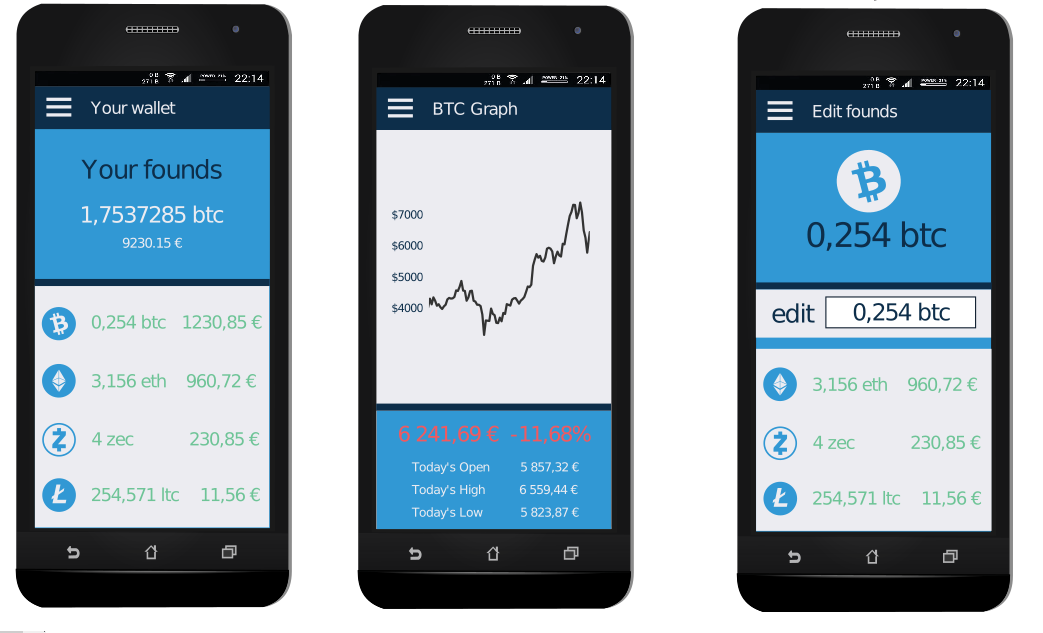
\includegraphics[width=0.8\columnwidth]{mockup}
	\end{center}
	\caption{Crypto finance tracker}
	\label{fig:mockup}
\end{figure}

\section{Tehnične funkcionalnosti}

\begin{itemize}
	\item Aplikacija bo vnešene količine kripto valut shranila v lokalno podatkovno bazo.
	\item Aplikacija bo vrednosti tečajev, če bo to možno (imamo podatkovni prenos?) prenesla iz spleta s pomočjo CryptoCompare API \cite{ccapi}.
	\item V primeru, da aplikacija nima dostopa do spleta, bo dostopala do vrednosti, ki jih je pridobila v zadnji seji. Te vrednosti bodo zapisane v lokalni bazi.
	\item Podprt bo izvoz in uvoz podatkovne baze na lokalni pomnilnik.
\end{itemize}


\begin{thebibliography}{9}
	
	\bibitem{ccapi}
	CryptoCompare API
	\url{https://www.cryptocompare.com/api/#introduction}
	[Dostopano 15.12.2017]
	
	
\end{thebibliography}

\end{document}  




